%
% approximation.tex
%
% (c) 2020 Prof Dr Andreas Müller, Hochschule Rapperswil
%
\subsection{Approximation
\label{pde:fem:subsection:approximation}}
\index{Approximation}%
Das äquivalente Minimalproblem zu einer partiellen Differentialgleichung
hat das Problem etwas vereinfacht, die Ordnung der Ableitung ist
reduziert worden, aber ist ist immer noch ein Problem, in dem eine
Funktion bestimmt werden muss, also ein unendlichdimensionales Problem.
In dieser Form ist es daher immer noch nicht einer effizienten
numerischen Lösung zugänglich.

\subsubsection{Beispielproblem}
Zur Illustration soll in diesem Abschnitt das folgende Problem 
gelöst werden.
Auf dem Interval $\Omega=[0,\pi]$ ist eine Funktion $f(x)$ gegeben.
Gesucht ist eine Funktion $u\colon [0,\pi]\to\mathbb R$ derart, dass
\begin{equation}
\begin{aligned}
u''(x) &= f(x)
\\
u(0) &= u_0 & u(\pi)&= u_1.
\end{aligned}
\label{buch:pde:approx:beispiel}
\end{equation}
Als erstes müssen wir das äquivalente Minimalproblem finden.

\begin{problem}
Sei $F(x)$ eine Stammfunktion von $f(x)$.
\index{Stammfunktion}%
Eine Lösung des Differentialgleichungsproblems~\eqref{buch:pde:approx:beispiel}
minimiert
\[
I(u)
=
\int_0^\pi (u'(x) - F(x))^2\,dx.
\]
\end{problem}

\begin{proof}[Beweis]
Die Richtungsableitung von $I(u)$ ist
\begin{align*}
\frac{dI}{d\varepsilon}(u+\varepsilon h)\bigg|_{\varepsilon=0}
&=
\int_0^\pi
2(u'(x)+\varepsilon h'(x)-F(x)) h'(x) 
\,dx
\\
&=
2
\int_0^\pi
(
u'(x)
-
F(x)
)
h'(x)
\,dx
\\
&=
2\biggl[(u'(x)-F(x))h(x)\biggr]_0^\pi
-
2\int_0^\pi
(u''(x)
-
F'(x))
h(x)
\,dx.
\intertext{Der erste Term verschwindet wegen $h(0)=h(\pi)=0$ und es bleibt}
&=
2\int_0^\pi
(u''(x)
-
f(x))
h(x)
\,dx
=0.
\end{align*}
Dies muss für alle $h(x)$ gelten, so dass folgt
$u''(x) -f(x)=0$ oder $u''(x)=f(x)$.
\end{proof}

Die Stammfunktion $F(x)$ ist nicht eindeutig bestimmt, vielmehr
ist jede $F(x)+C$ ebenfalls eine Stammfunktion.
Nach obiger Rechnung führt sie jedoch auf die gleichen Minima.

\subsubsection{Approximation mit Polynomen}
\index{Approximation durch Polynome}
Wir können aber davon ausgehen, dass die Lösungsfunktionen einigermassen
glatt sind, also sich gut durch ein Polynom approximieren lässt.
Wir approximieren jetzt $u(x)$ als Polynom und schreiben
\[
u(x) = a_0 + a_1x + a_2x^2 + \dots + a_nx^n.
\]
Das Minimalprinzip für $u(x)$ führt auf ein Minimalprinzip für 
die Koeffizienten $a_k$.
\index{Minimalprinzip}%
Zunächst brauchen wir die Ableitung von $u(x)$:
\begin{align*}
u'(x) &= \sum_{k=1}^n ka_kx^{k-1}.
\end{align*}
Jetzt müssen wir das Integral von
\begin{equation}
(u'(x)-F(x))^2
=
u'(x)^2 - 2u'(x)F(x) + F(x)^2
\label{buch:fem:integrand}
\end{equation}
durch 
die Koeffizienten $a_k$ ausdrücken.
Für die drei Terme rechts in \eqref{buch:fem:integrand} müssen die Integrale
\begin{align*}
\int_0^\pi u'(x)^2\,dx
&=
\int_0^\pi
\sum_{i,j=1}^n ija_ia_jx^{i+j-2}
\,dx
=
\sum_{i,j=1}^n ij \int_0^\pi x^{i+j-2}\,dx\, a_ia_j
=
\sum_{i,j=1}^n
\underbrace{ij \frac{\pi^{i+j-1}}{i+j-1}}_{\displaystyle b_{ij}}
a_ia_j
=
a^tBa
\\
\int_0^\pi u(x)'F(x) \,dx
&=
\int_0^\pi \sum_{i=1}^n ia_i x^{i-1} F(x) \,dx
=
\sum_{i=1}^n
a_i
\underbrace{\int_0^\pi 
ix^{i-1} F(x)\,dx}_{\displaystyle =b_i}
=
b^t a
\\
\int_0^\pi F(x)^2\,dx &=: c
\end{align*}
ausgewertet werden können.
Gesucht ist jetzt also ein Koeffizientenvektor $a$, der den Ausdruck
\index{Koeffizientenvektor}%
\[
Q(a) = a^t B a + b^t a + c
\]
minimiert.
Der Summand $c$ kann natürlich weggelassen werden.

Die Randbedingungen müssen natürlich auch erfüllt sein, auch
diese können wir durch die Polynomkoeffizienten ausdrücken:
\begin{align*}
u_0=u(0)   &= a_0
\\
u_1=u(\pi) &= a_0 + a_1\pi + a_2\pi^2+\dots a_n\pi^n.
\end{align*}
Dies lässt sich auch in Matrixform mit der Matrix
\[
A=\begin{pmatrix}
1&0&0&\dots&0\\
1&\pi&\pi^2&\dots&\pi^n
\end{pmatrix}
\]
als
\[
Aa = \begin{pmatrix}u_0\\u_1\end{pmatrix}
\]
schreiben.

Wir machen das Problem noch etwas konkreter und verlangen $f(x)=1$
und $u_0=u_1=0$.
Dann ist $F(x)=x$ eine mögliche Stammfunktion und damit lässt sich
der Vektor $b$ berechnen als
\[
b_i
=
\int_0^\pi i F(x) x^{i-1}\,dx
=
\int_0^\pi i x^i\,dx
=
\frac{i}{i+1}
\pi^{i+1}.
\]
Die Matrix $B$ ist
\begin{align*}
B&=\begin{pmatrix}
\pi   & \pi^2            & \pi^3            \\
\pi^2 & \frac{4}{3}\pi^3 & \frac{3}{2}\pi^4 \\
\pi^3 & \frac{3}{2}\pi^4 & \frac{9}{5}\pi^5
\end{pmatrix}.
\end{align*}
Aus den Randbedingung folgt $a_0=0$ und
\[
a_1\pi+a_2\pi^2=0
\qquad\Rightarrow\qquad
a_1 = \pi a_2.
\]
Die gesuchte Lösung muss sich also den Ausdruck
\[
a_2
\begin{pmatrix}
1\\\pi
\end{pmatrix}^t
\pi^3
\begin{pmatrix}
\frac43   &\frac32\pi\\
\frac32\pi&\frac95\pi^2
\end{pmatrix}
\begin{pmatrix}
1\\\pi
\end{pmatrix}
a_2
-
\begin{pmatrix}
\frac23\pi^3\\\frac34\pi^4
\end{pmatrix}
\begin{pmatrix}
1\\\pi
\end{pmatrix}
a_2
=
\biggl(
\frac43\pi^3+3\pi^5 +\frac95\pi^7
\biggr)
a_2^2
-\biggl(\frac23\pi^3+\frac34\pi^5\biggr)
a^2.
\]
Gesucht wird also nur das Minimum eines quadratischen Ausdrucks 
in $a_2$ und dieses wird bei $a_2=\frac12$ angenommen.
Tatsächlich kann man nachprüfen, dass
\[
u(x)
=
\frac12\biggl(x-\frac{\pi}2\biggr)^2 -\frac{\pi^2}8
=
\frac12x^2 -\frac12 x\pi +\frac{\pi^2}8 - \frac{\pi^2}8
=
\frac12x\biggl(x-\frac{\pi}2\biggr)
\]
eine Lösung des Problems ist.

\subsubsection{Allgemeine Formulierung}
Etwas allgemeiner kann man das Problem wie folgt formulieren.
Gesucht sei die Lösung der Differentialgleichung $u''(x)=f(x)$ auf
dem Intervall $[a,b]$ mit Randbedingungen $u(a)=u_0$ und $u(b)=u_1$.
Das zugehörige Minimalprinzip verlangt, dass
\[
I(u) = \int_a^b (u'(x) - F(x))^2\,dx,
\qquad \text{mit}\qquad F(x) = \int_a^x f(\xi)\,d\xi
\]
minimiert wird mit der Nebenbedingungen $u(a)=u_0$ und $u(b)=u_1$.
Gesucht ist die Lösung $u(x)$ als Linearkombination einer linear
unabhängigen Menge von Funktionen
$\varphi_0(x),\varphi_1(x),\dots,\varphi_n(x)$.
Zu bestimmen sind die Koeffizienten $a_k\in\mathbb R$ der Linearkombination
\[
u(x) = a_0\varphi_0(x) + a_1\varphi_1(x) + \dots + a_n\varphi_n(x)
=
\sum_{k=0}^n a_k\varphi_k(x).
\]
Das Minimalprinzip kann durch die Koeffizienten $a_k$ als
\begin{align*}
\int_a^b (u'(x)-F(x))^2 \,dx
&=
\int_a^b 
\sum_{i,j=0}^n
a_ia_j
\varphi'_i(x)\varphi'_j(x) 
-2F(x)
\sum_{i=0}^n \varphi'_i(x)
+
F(x)^2
\,dx
\\
&=
\sum_{i,j=0}^n a_ia_j
\underbrace{\int_a^b \varphi'_i(x)\varphi'_j(x)\,dx}_{\displaystyle=b_{ij}}
+
\sum_{i=0}^n a_k \underbrace{\int_a^b \varphi_i'(x)F(x)\,dx }_{\displaystyle=c_i}
+
\int_a^b F(x)^2\,dx
\end{align*}
ausgedrückt werden.
Der letzte Summand hat keinen Einfluss auf das Minimum und kann daher
weggelassen werden.
Die Randbedingungen können ebenfalls vektoriell geschrieben werden:
\[
\left.
\begin{aligned}
u_0&=u(a) = \sum_{i=0}^n a_i\varphi_i(a) \\
u_1&=u(b) = \sum_{i=0}^n a_i\varphi_i(b)
\end{aligned}
\quad
\right\}
\qquad\Rightarrow\qquad
\underbrace{\begin{pmatrix}
\varphi_0(a)& \varphi_1(a) & \dots & \varphi_n(a) \\
\varphi_0(b)& \varphi_1(b) & \dots & \varphi_n(b) \\
\end{pmatrix}}_{\displaystyle =A}
\begin{pmatrix}a_0\\\vdots\\a_n\end{pmatrix}
=
\begin{pmatrix}
u_0\\u_1
\end{pmatrix} = b
\]
Das Problem ist damit auf das quadratische Minimalproblem
\index{quadratisches Minimalproblem}%
\[
\begin{aligned}
&\text{minimiere}&
Q(a) &= a^tBa + c^ta 
\\
&\text{Nebenbedingung:}&
Aa&=b
\end{aligned}
\]
mit der Matrix
\[
B=(b_{ij})
\quad\text{mit}\quad
b_{ij}
= 
\int_a^b \varphi'_i(x)\varphi'_j(x)\,dx
\]
und dem Vektor
\[
c=(c_i)
\quad
\text{mit}\quad
c_i
=
\int_a^b \varphi_i'(x) F(x)\,dx
\]
zurückgeführt.

\subsubsection{Höhere Dimensionen}
Das Beispielproblem der vorangegangenen Abschnitte war eindimensional,
was erlaubt hat, bekannte Formeln wie die partielle Integration aus der
Analysis zu verwenden.
Ziel dieses Abschnitts ist, ein paar Eigenheiten der Verallgemeinerung
auf ein mehrdimensionales Problem zu diskutieren.

Sei $\Omega\subset\mathbb R^2$ ein zweidimensionales Gebiet mit glattem
Rand $\partial \Omega$,
zum Beispiel ein Rechteck wie in Abbildung~\ref{buch:pde:pfadintegral}.
%Es ist klar, dass dies auch auf höhere Dimensionen verallgemeinert werden.
Ausserdem ist $f\colon\Omega\to\mathbb R$ und
$g\colon\partial\Omega\to\mathbb R$ geben.
Das Differentialgleichungsproblem sucht
eine Funktion $u\colon\overline{\Omega}\to\mathbb R$ mit
\begin{equation}
\begin{aligned}
\Delta u&=f &&\text{in $\Omega$}
\\
u&=g&&\text{auf $\partial\Omega$}.
\end{aligned}
\label{buch:pde:eqn:dgl2d}
\end{equation}
Die Rechnung zum eindimensionalen Problem suggeriert, dass 
das äquivalente Minimalproblem 
\begin{equation}
I(u)
=
\int_{\Omega} (\nabla u(x,y) - F(x,y))^2\,dx\,dy
\label{buch:pde:eqn:minimal2d}
\end{equation}
ist, wobei $F(x,y)$ eine beliebige vektorwertige Funktion mit
$\nabla\cdot F(x,y) = f(x,y)$ ist.

In den meisten Fällen ist es einfach, eine solche Funktion zu
finden.
Besonders einfach ist es, wenn die Funktion $f\colon\Omega\to\mathbb R$
stetig zu einer Funktion $\bar{f}\colon\mathbb R^2\to R$ ausgedehnt
werden kann.
Dies ist nicht immer möglich, wie die Funktion $\varphi$ des Polarwinkels
des Punktes $(x,y)$ auf dem Gebiet von
Abbildung~\ref{buch:pde:figure:ringgebiet} zeigt.
\index{Polarwinkel}%
\begin{figure}
\centering
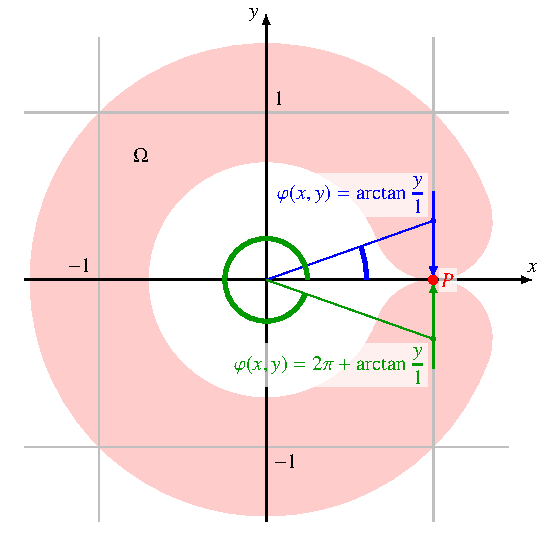
\includegraphics{chapters/70-pde/images/ringgebiet.pdf}
\caption{Die auf dem Gebiet $\Omega$ definiert Funktion, $\varphi$,
die einem Punkt den Polarwinkel $\varphi$ in Polarkoordinaten zuordnet,
kann nicht stetig auf ganz $\mathbb R^2$ ausgedehnt werden.
\index{Polarkoordinaten}%
Der Grund dafür sind die unterschiedlichen Grenzwert im Punkt $P$.
\label{buch:pde:figure:ringgebiet}}
\end{figure}
Gäbe es eine stetige Funktion $\bar{\varphi}$, die $\varphi$ erweitert, dann
müssten die Grenzwerte von $\bar{\varphi}$ im Punkt $P$ von ``oben'' und
von ``unten'' übereinstimmen.
Der Grenzwert im Punkt $P$ hängt aber von der Richtung ab,
es ist
\begin{align*}
\lim_{y\to 0+}\varphi(1,y) &= \lim_{y\to 0+}\arctan\frac{y}{1} = 0
\\
\lim_{y\to 0-}\varphi(1,y) &= 2\pi + \lim_{y\to 0-}\arctan\frac{-y}{1} = 2\pi.
\end{align*}
Die Grenzwerte sind also verschieden.

Nehmen wir jetzt also an, dass es eine stetige Funktion
$\bar{f}\colon\mathbb R^2\to\mathbb R$ gibt mit $\bar{f}(x,y)=f(x,y)$
für $(x,y)\in\Omega$.
Wir betrachten die Vektorfunktion $F(x,y)$ mit Komponenten
\begin{equation}
\left.
\begin{aligned}
F_x(x,y) &= \int_0^x \bar{f}(\xi, y)\,d\xi \\
F_y(x,y) &= 0
\end{aligned}
\quad
\right\}
\qquad\Rightarrow\qquad
F(x,y)
=
\begin{pmatrix}F_x(x,y)\\F_y(x,y)\end{pmatrix}
=
\begin{pmatrix}F_x(x,y)\\0\end{pmatrix}.
\label{buch:pde:eqn:divFf}
\end{equation}
Die Divergenz von $F(x,y)$ ist
\begin{align*}
\nabla\cdot F(x,y)
=
\frac{\partial F_x}{\partial x}(x,y)
+
\frac{\partial F_y}{\partial y}(x,y)
=
\frac{\partial}{\partial x}
\int_0^x \bar{f}(\xi, y)\,d\xi
=
f(x,y).
\end{align*}
Die Funktion $F(x,y)$ definiert in \eqref{buch:pde:eqn:divFf}
ist also eine Funktion der gesuchten Art.
Die Erweiterbarkeit der Funktion $f(x,y)$ auf $\bar{f}(x,y)$ 
stellt sicher, dass das Integral und damit $F(x,y)$ eine stetige Funktion
von $x$ und $y$ wird, so dass das Minimalproblem wohldefiniert ist.

Für das vorgeschlagene Minimalprinzip können wir jetzt wieder die
Richtungsableitung für eine Änderung von $u$ um eine Funktion $h$
mit verschwindenden Randwerten berechnen.
\index{Richtungsableitung}%
Wie früher finden wir
\begin{align*}
\frac{dI(u+\varepsilon h)}{d\varepsilon}\bigg|_{\varepsilon=0}
&=
\int_\Omega 2(\nabla u(x,y) -F(x,y))\cdot \nabla h(x,y)\,dx\,dy
\\
&=
\int_{\partial\Omega} (\nabla u(x,y) - F(x,y))h(x,y)\cdot d\vec{n}
-
\int_{\Omega} (\Delta u(x,y) -\nabla F(x,y)) h(x,y) \,dx\,dy
\intertext{Darin verschwindet der erste Term, da $h(x,y)=0$ ist auf dem Rand.
Es bleibt}
&=
-
\int_{\Omega} (\Delta u(x,y) - f(x,y)) h(x,y) \,dx\,dy.
\end{align*}
Da dieser Ausdruck für jede Funktion $h$ mit $h(x,y)=0$ mit
$(x,y)\in\partial\Omega$
verschwinden muss, folgt wieder, dass
\[
\Delta u = f
\]
in $\Omega$ gelten muss.
Das Minimalprinzip~\eqref{buch:pde:eqn:minimal2d} gehört also tatsächlich
zur Differentialgleichung~\eqref{buch:pde:eqn:dgl2d}.

%Für die Ausdehnbarkeit der Funktion $f$ vom Gebiet $\Omega$ mit glattem Rand
%auf $\mathbb R^2$ genügt es, dass sich $f$ stetig auf den Rand
%$\partial \Omega$ fortsetzen.
%Damit werden Fälle wie das Beispiel in
%Abbildung~\ref{buch:pde:figure:ringgebiet}
%bereits ausgeschlossen.



